
\section{供应商的选择}

通过分析过去五年内,生产企业向402家原材料供货商发起的订单数据,可发现其中一些更受该企业青睐,该企业在相同周期里向这些供应商发出更多订单。
与之相反,也有一些供应商参与原材料供应较少。
%这里最好插一张展示供货商供货能力的图片
因此,为了制定该企业的最优订货策略,有必要筛选出对原材料供应影响较大的供应商,并减少对供应影响较少供应商的依赖。

与此同时,订货法案还受到供货商数量的影响,过多的供应商需要花费企业更多的成本,而且到货的不稳定因素增多,进而有可能影响企业的生产计划;供应商数量过少,虽然能够降低管理成本和订货成本,但是到货的时间和质量的风险增大,从风险规避的角度来说,供应商数量应该维持在高水平状态\cite{顾丽娟2014基于最优供应商数量的补货策略研究}。

综上所述,筛选出供应影响力较强的供应商,并结合生产需求选择合适数量的供应商,与之建立长期、稳定的合作供给关系,能够显著降低该企业的管理成本和资金链风险。
因此,本文通过量化分析供货特征和提出假设,建立并求解相应评价模型,为生产企业订购决策提供基础和指导。%需修改


% 上述企业近5年共与402家原材料供应商有订货交易:从供货量数据来看,供货商有着不同的供货特征,对生产企业的重要性也不一样;从订货量数据来看,生产企业对供货商有所偏好,但在订购原材料时,还是有比较混乱的情况产生。
% 事实上,生产企业往往会与对其比较重要的原材料供应商形成商业伙伴,寻求长久稳定而优质的合作关系。
% 显然,生产企业难以同几百家供应商始终保持高质量的合作关系,但商业伙伴过少也是不利的,这会导致供货不足或不稳。
% 本节便是希望通过对供货商的供货特征进行量化分析,进而建立评价模型,在满足对生产企业的原材料供应出租且稳定时,选出最少但最重要的供应商,来为生产企业进行商业合作提供理论指导。

\subsection{指标的选取}

为了对供应商的的供货特征进行量化分析,建立合理的评价模型,本文首先选取了以下的指标:
\begin{enumerate}

\item 订货次数$N_j$:

订货次数表示供应商过去5年向生产企业供货的次数,直接反映出该企业对其的依赖程度。
订货次数$N_j$越大,表示企业对该供应商越认可。
\begin{equation}
    \nu_{ij}=
\begin{cases}
0,& \text{供应商S$j$在第$i$ 周没有订单,}
\\
1,& \text{供应商S$j$在第$i$ 周接到订单;}
\end{cases}
\end{equation}
\noindent 上式中,$\nu_{ij}$是表示某供应商在该周是否接到订单的逻辑变量。通过累加求和,得到定货次数
\begin{equation}
    N_j=\sum_{i=001}^{240}\nu_{ij}.
\end{equation}

\item 供应商S$j(j=001,002,\cdots,402)$近五年企业的订货总量$\varkappa_j$

企业会向重要的供货商订购大量货物。$\varkappa_j$大的供应商更受企业欢迎,对企业的重要性强。对于供应商S$j$,有
\begin{equation}
    \varkappa_j=\sum_{i=001}^{240}\chi_{ij},
\end{equation}
其中,$\chi_{ij}$是第$i$周,供货商S$j$接到的订货量。

\item 供应商S$j(j=001,002,\cdots,402)$近五年企业的供货总量$\Psi_j$

供应商的供货量能反映供货量的供应能力,供应能力强的供货商能有力地保障企业生产,所以$\Psi_j$越大,相应的供货商越重要,与$\varkappa_j$类似
\begin{equation}
    \Psi_j=\sum_{i=001}^{240}\psi_{ij},
\end{equation}
其中,$\psi_{ij}$是第$i$周,供货商S$j$对企业的供货量。

\item 平均供货偏差$\varepsilon_j$:

对企业来讲,越能按照订货量进行供货的供应商是越优质的。我们选择供货量和订货量的差占订货量的比值,表征供货偏差,即供应商S$j$在第$i$周的供货偏差为
\begin{equation}
    \varepsilon_{ij}=\frac{\chi_{ij}-\psi_{ij}}{\chi_{ij}},
\end{equation}
而平均供货偏差$\varepsilon_j$应为$\varepsilon_{ij}$的绝对值的平均值,即
\begin{equation}
    \varepsilon_j=\frac{\sum_{i=001}^{240}|\varepsilon_{ij}|}{N_j}.
\end{equation}

进而本文得到了供应商在供货时绝对偏差量的期望值
\begin{equation}
    E_j=\chi_{ij} \times \varepsilon_j.
\end{equation}

\item 单次最大供应量$\Psi'_j$:

如果供应商能一次性向企业提供大量原材料,其就能在一定程度上向企业证明其的供应能力强大,更适合成为对于企业重要的供应商。
即单次最大供应量$\Psi'_j$越大,相对的供应商越重要
\begin{equation}
    \Psi'_j=max \{ \psi_{1j},\psi_{2j},\dots,\psi_{240j} \}.
\end{equation}

\end{enumerate}

\subsection{基于熵权的TOPSIS方法选优}
\label{选优}
% 以上共遴选了5个指标,本文希望综合考虑之,进而完成对于供应商的的供货特征的量化分析。
% 从主观上讲,平均供货偏差应当在以上四个指标中起到最为重要的作用;相对地,供货偏差方差的影响则不如平均供货偏差显著。

根据过去五年的交易数据,本文建立了基于熵权法的理想解法供应商评价体系,并根据评价得分选出供应影响力较强的供应商。

理想解法亦称TOPSIS法,是一种有效的多指标评价方法。
理想解法通过构造评价问题的正、负理想解,根据每个供应商到理想供应商的相对贴近度,即控制靠近正理想解或远离负理想解的程度,来对方案进行排序,以选出最优方案。

TOPSIS法对样本数据无特殊要求,并且能清晰地反映各方案的差距,被广泛应用于多方案多目标的决策评价\cite{金王莉2018基于熵权},但使用TOPSIS法之前必须确定各评价指标的权重系数。

在传统评价模型的应用过程中,由于指标权重难以确定,使用场景有很大的局限性。
而常见的多要素问题中指标权重的确定方法有:专家评测法、层次分析法、二向系数法、熵值法、环比分析法、模糊聚类分析法等。
由于前三种方法存在着较大的主观因素,而最后一种方法主要用于模糊指标的重要程度分类,为提高综合评价的准确性和客观性,本文故采用熵权法来解决供应商评价选优模型中的权重赋值问题\cite{供应链}。


熵权法是一种客观赋权方法。
在具体使用过程中,熵权法根据各指标的变异程度,利用信息熵计算出各指标的熵权,从而得出较为客观的指标权重。


\subsubsection{权重计算}

\begin{enumerate}

\item 构造原始数据矩阵

${\text{\bf A}}={(a_{jk})}_{402 \times 5}$(用$a_{jk}$指代各供应商的评价值),将以上五个指标放入以下矩阵。
\begin{equation}       %开始数学环境
\left(                 %左括号
  \begin{array}{cccc}
    W_1 & W_2 & \dots & W_{402}\\
    \varkappa_1 & \varkappa_2 & \dots & \varkappa_402\\
    \Psi_1 & \Psi_2 & \dots & \Psi_402\\
    \varepsilon_1 & \varepsilon_2 & \dots & \varepsilon_402 \\
    N_1 & N_2 & \dots & N_402 \\
  \end{array}
\right)                 %右括号
\end{equation}

\item 规范化属性值

得到数据矩阵$\bf B$ $ =(b_{jk})_{402 \times 5}$,为了使每个属性变换后的最优值为1,且最差值为0,这里先进行0—1标准化
\begin{equation}
    b'_{jk}=\frac{b_{jk}-b_{min}}{b_{max}-b_{min}}.
\end{equation}

此外,为了减小矩阵中的订货量和供货量波动过大的影响,对其进行对数化处理。重新赋值,得
\begin{equation}
    b''_{jk}=\ln b'_{jk} (k=1,2,5).
\end{equation}

\item 利用数据矩阵

计算$p_{jk}(k=1,2,3,4,5)$,即第$j$家供应商关于第$k$个指标值的比重
\begin{equation}
    p_{jk}=\frac{b''_{jk}}{\sum_{j=1}^{402}b''_{jk}}.
\end{equation}

\item 计算第$k$项指标的熵值

熵本源于热力学与统计物理,后由香农引入信息论。根据熵的定义,有
\begin{equation}
    e_k=-\frac{1}{ln402}\sum_{j=1}^{402}p_{jk}lnp_{jk}.
\end{equation}

\item 计算第$k$指标的变异系数

\begin{equation}
    g_k=1-e_k,
\end{equation}
对于第$k$项指标,$e_k$越大,指标值的变异程度就越小。

\item 计算第$k$指标的权重

\begin{equation}
    \omega_k=\frac{g_k}{\sum_{k=1}^{5}g_k}.
\end{equation}

\end{enumerate}

\subsubsection{供应商评价}

\begin{enumerate}

\item 用向量规划化的方法求得规范决策矩阵
\begin{equation}
 {\bf \breve{B}} =(\breve{b}_{jk})_{402 \times 5},
\end{equation}
其中
\begin{equation}
    \breve{b}_{jk}=\frac{{b''}_{jk}}{\sqrt{\sum_{j=1}^{402}{b''}_{jk}^2}}.
\end{equation}
\item 构造加权规范阵$ \bf \check{B} $ $=(\check{b}_{jk})_{402 \times 5}$

凭借熵权法给定的各属性的权重,得权重向量$ \bf \Omega $ $ =(\omega_1,\omega_2,\omega_3,\omega_4,\omega_5)$,则有
\begin{equation}
    \check{b}_{jk}=\omega_k\breve{b}_{jk}.
\end{equation}
\item 确定正、负理想解$ \bf C^+$ $=(c_1^+,c_2^+,c_3^+,c_4^+,c_5^+)$
、
${\bf C^{-}}=(c_1^-,c_2^-,c_3^-,c_4^-,c_5^-)$

正理想解
\begin{equation}
c_{k}^{+}=\left\{\begin{array}{ll}
{ }_{\ j}^{\max } \check{b}_{jk}, & k \text { 为效益型属性 }, \\
{ }_{\ j}^{\min } \check{b}_{jk}, & k \text { 为成本型属性 };
\end{array}\right.
\end{equation}
负理想解反之。

\item 计算各供应商与正、负理想解的距离

与正理想解的距离
\begin{equation}
    s_j^+=\sqrt{\sum_{k=1}^5(\check{b}_{jk}-c_k^+)^2} ,
\end{equation}
与负理想解的距离同理。
\item 计算各供应商对理想解的相对接近程度作排序指标值(即综合评价指数)
\begin{equation}
    f_j=\frac{s_j^-}{s_j^-+s_j^+}.
\end{equation}
\item 按$f_j$由大到小排列供应商的优劣次序

\end{enumerate}

\subsection{供应商的评价结果}

\subsubsection{各个指标的权重}

运用熵权法,对过去交易数据进行分析,得到各个特征指标的权重,如图 1 所示。

\begin{center} {\centering
\vbox{

	\centerline{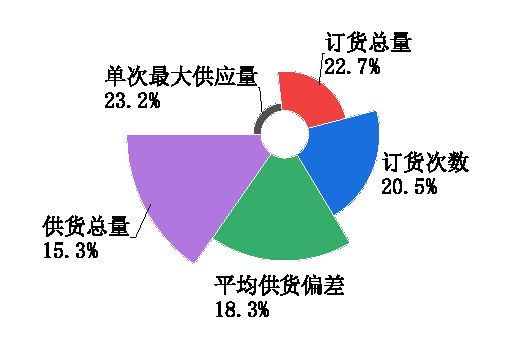
\includegraphics[width=8cm]{Image/Graph2.eps}}
	\vskip 1mm{\small
	图1\quad 各指标权重
	\\}
	}
	}
\end{center}

\subsubsection{供应商综合评价指数}

根据评价指标和上文计算出的权重,对供应商进行评价,表1是各供应商的综合评价得分。
% \begin{multicols}{2}%开始双栏显示

\begin{center} {\centering
\vbox{
	\centerline{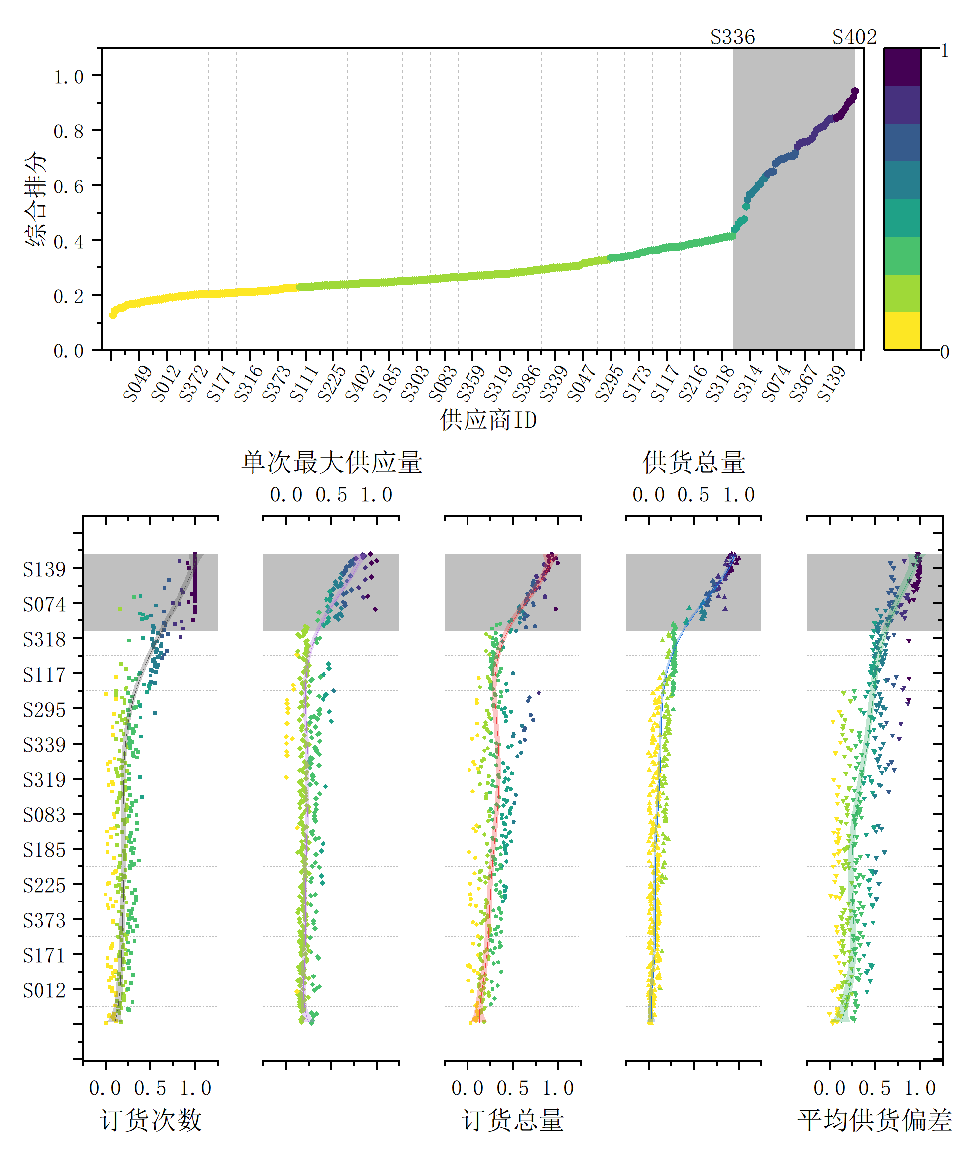
\includegraphics[width=16cm]{Image/评价总览.eps}}
	\vskip 1mm{\small
	图1\quad 各指标权重
	\\}
	}
	}
\vbox{\centering{\small 表1\quad 排名前十八名的供应商评价分数
\\
Table 1 \quad Weights of each indicator } \vskip2mm
\renewcommand{\baselinestretch}{1.2}
{\footnotesize\centerline{\tabcolsep=22pt\begin{tabular*}{\textwidth}{cccccc}
        \toprule
       供应商&  订货次数 & 订货总量 & 供货总量 & 平均供货偏差 & 单次最大供应量\\
        \midrule
        0	& 91	&350	&74.24242424	&0.837362637	&9.090909091\\
        1	& 95	&515	&455	&0.490977444	&111.6666667\\
        2	& 199&	19831.94444	&18247.22222	&0.206018934	&537.5\\
        3	& 103&	1080.30303	&96.96969697	&0.794073047	&12.12121212\\
        4	& 114&	10896.66667	&11520	&0.171227722	&213.3333333\\
        5	& 55	&641.6666667	&41.66666667&	0.871212121&	6.944444444\\
        6	& 240&	11193.33333	&11580&	0.379053947	&258.3333333\\
        7	& 56	&130.5555556	&56.94444444	&0.776785714&	18.05555556\\
        8	& 80	&1083.333333	&46.96969697	&0.81125	&6.060606061\\
        9	& 88	&872.7272727	&257.5757576	&0.746306818&	45.45454545\\
        10	& 43	&116.6666667	&118.0555556	&0.494601329	&15.27777778\\
        11	& 68	&513.3333333	&48.33333333	&0.907352941	&10\\
        12	& 29	&61.11111111	&61.11111111	&0.562931034&	12.5\\
        13	& 27	&53.33333333	&46.66666667	&0.574074074&	5\\
        14	& 54	&46471.66667	&46.66666667	&0.808641975&	6.666666667\\
        15	& 22	&63.33333333	&61.66666667	&0.315909091&	11.66666667\\
        16	& 67	&323.3333333	&230	&0.710465529	&41.66666667\\
        17	& 72	&171.2121212	&100	&0.740625	&10.60606061\\

        \bottomrule
\end{tabular*}}}}\end{center}

\subsubsection{供应商的预选}

根据以上评价模型对于各供应商的得分,将供应商由高到低排序,并分别以各供应商及其评价分数为、横坐标,绘制图像。
由图2可见,供应商的得分状况呈积聚分布,并且在0.416分处,有显著的拐点。
因此,本文先根据评价分数,首先筛选出66家高分供应商。


\subsection{供应商数量优化}

通过预选供应商,本文已筛选出供应能力较突出的供应商。
为了进一步得到合适数量的供应商,满足企业每周生产需求,并使供货最稳定,本文建立供应商选择0\textendash1规划模型,以决定实际供货商选取:
% \begin{equation}
%     \lambda_j=
% \begin{cases}
% 0& \text{第$j$家供应商未选上}
% \\
% 1& \text{第$j$家供应商被选上}
% \end{cases}
% \end{equation}
\begin{equation}
\begin{split}
{\bf min}\quad &\Lambda=\sum_{j=1}^{66} \lambda_j\varepsilon_j \\
{\bf s.t.}\quad &\sum_{j=1}^{66} \lambda_j\bar{y}_j > 2.84\times 10^4
\end{split}
\end{equation}
其中,$\lambda_j$是表示第$j$家供应商是否被选上的0\textendash1变量,而$\bar{y}_j$表示第$j$家供应商的供货能力,计算方法见于后文。
通过对模型的求解,得到最终选定的44家供应商。
综上所述,本文认为该企业应至少选择44家供应商供应原材料才可能满足生产的需求。
